\setchapterimage[6.5cm]{neuron}
\setchapterpreamble[u]{\margintoc}
\chapter[Neural networks]{Neural networks\footnotemark[0]}


%====================================================================================================
\section{History}

%----------------------------------------------------------------------------------------------------
\subsection{Biological inspiration}
Artificial neural networks were originaly created as a way of modeling behavior of biological
neurons.
Neurons are at their core cells so most of metabolic processes common for animal cells also
occur in them. However just like red blood cells neural cells do not divide on their own and new
neurons are generated by specialised stem cells.
\begin{figure}[hb]
	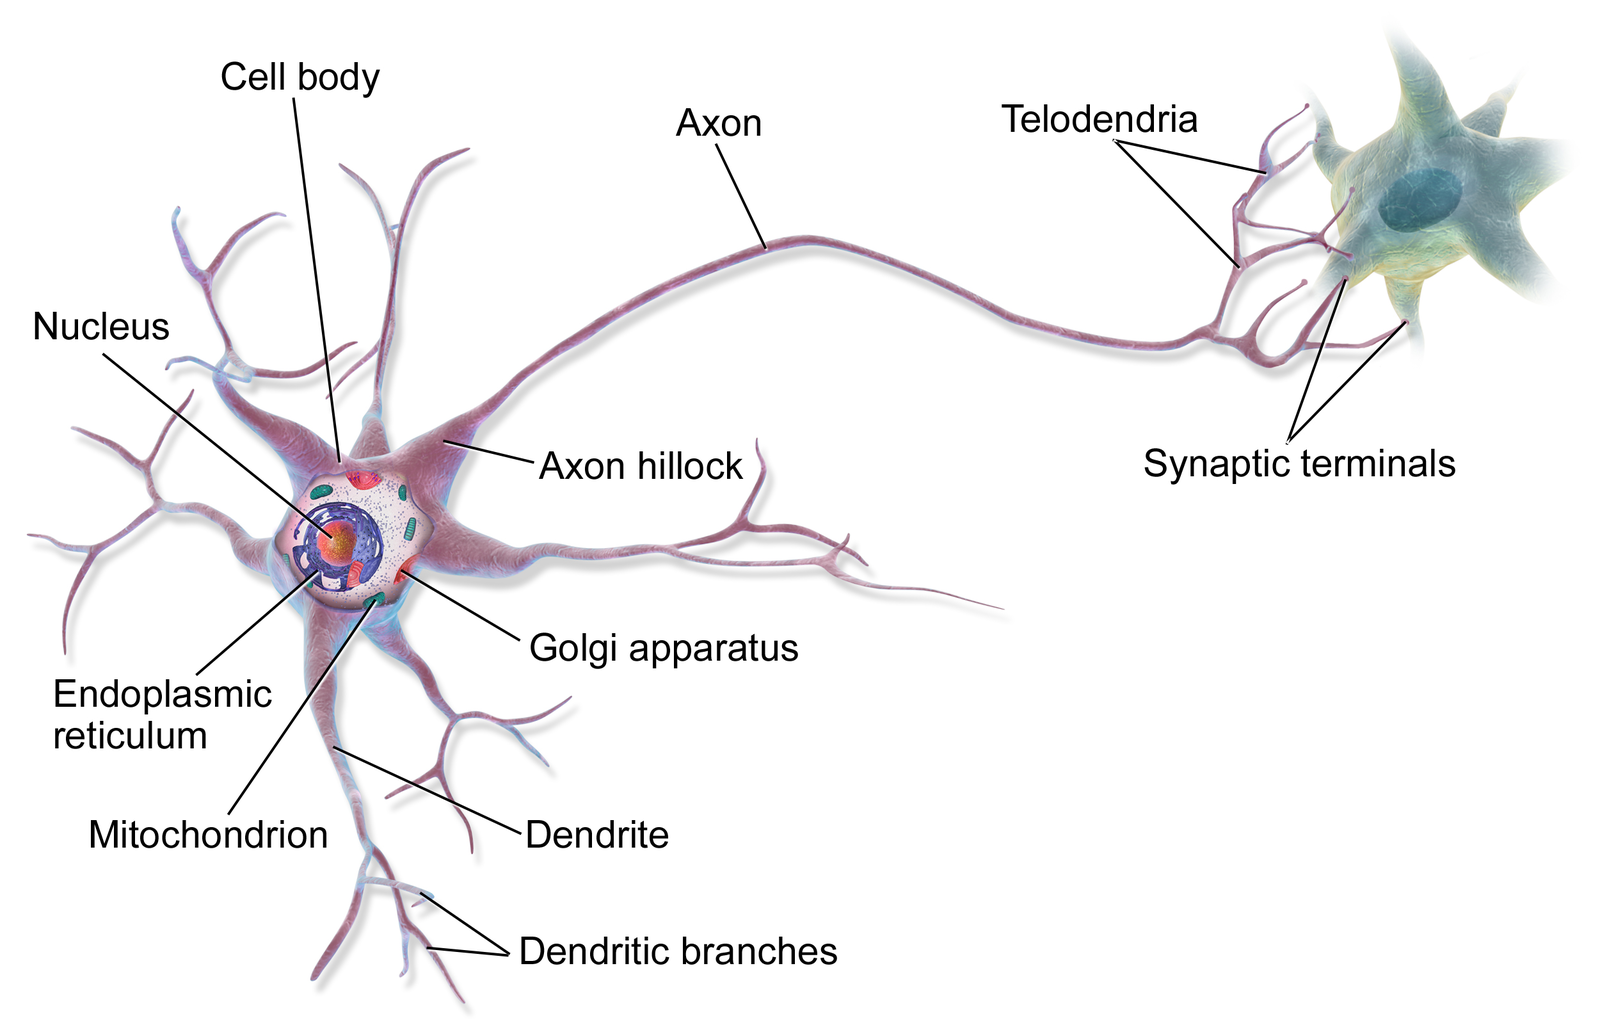
\includegraphics[width=\textwidth]{Blausen_MultipolarNeuron}
	\caption{Neural cell structure. Image by Bruce Blaus}
	\labfig{fig:Blausen-Neuron}
\end{figure}
There is however one behavior that until recently was believed to be specific to only neural cells
and even recent studies extend this ability to glial cells only.
This is ability to transfer a electric signal trough length of cell axon 

%----------------------------------------------------------------------------------------------------
\subsection{Cybernetics, first steps in modeling of neural systems}

%----------------------------------------------------------------------------------------------------
\subsection{Perceptron and first advent of neural networks}

%----------------------------------------------------------------------------------------------------
\subsection{Deep learning and second advent of neural networks}

%----------------------------------------------------------------------------------------------------
\subsection{Modern day}


%====================================================================================================
\section{Feed forward neural networks}

%----------------------------------------------------------------------------------------------------
\subsection{Mathematical model of neuron}
First mathematical model of the neural cell was created in 1943 by Warren MuCulloch and Walter Pitts.
It aimed at recreating an behavior of the neuron electric potenitial activation as a result of
synaptic potential reaching specific bias. What is important this model was never supposed to
precisely mimic behavior of biological neuron and as such do not include representation of metabolic
processes or even neurotransmition.
However despite significant simplification McCulloch-Pitts neuron proven to have many uses and
its basic structure were used to create most of modern day models.
Essentialy in this model neuron is a finction $f_n(x):\mathbb{R} \rightarrow \{ 0,1 \} $ where $n$
is size of input.
In such case equation describing neuron response is as follows:




%----------------------------------------------------------------------------------------------------
\subsection{Perceptron, abilities and limitations}

%----------------------------------------------------------------------------------------------------
\subsection{Multi layer neural networks}

%----------------------------------------------------------------------------------------------------
\subsection{Limitations on neural networks depth}


%====================================================================================================
\section{Recurrent networks and deep learning}

%----------------------------------------------------------------------------------------------------
\subsection{Deep learning models}

%----------------------------------------------------------------------------------------------------
\subsection{Simple recurrent networks}

%----------------------------------------------------------------------------------------------------
\subsection{Long short term memory networks}


\footnotetext{Chapter image from Pixbay, usage according to Pixbay licence
	\url{https://pixabay.com/illustrations/neurons-brain-cells-brain-structure-440660/}}
